\documentclass[12pt]{article}
\usepackage[margin=1in]{geometry}
\usepackage{graphicx}
\usepackage{float}
\usepackage{hyperref}
\usepackage{booktabs}
\usepackage{setspace}

\singlespacing

\title{Evaluating Classical Machine Learning for Real-Time EEG Attention State Classification on Budget Hardware}
\author{Data Science Project Report \\ CMPT 353}
\date{\today}

\begin{document}

\maketitle

\section{Introduction and Motivation}

I recently joined NeuraXtension, a neuroscience club at Simon Fraser University (SFU). As the club was exploring new projects, the idea of building an attention state classifier using electroencephalogram (EEG) data emerged. This concept deeply resonated with me and inspired the topic for this project. Specifically, I wanted to explore existing machine learning methods and their effectiveness in the context of consumer-grade, budget hardware. 

Modern BCI research often relies on medical-grade equipment with 32 to 64 electrodes sampling at high frequencies. However, our club is interested in the ``NeuroPawn,'' a budget EEG headset that features only 7 channels (F3, Fz, F4, C3, Cz, C4, Pz) and samples at 125 Hz. The central problem of this project is determining whether classical machine learning techniques can accurately classify human mental attention states (Focused vs. Unfocused) when restricted to the limited hardware specifications of a budget headset like the NeuroPawn.

\section{Data Acquisition and the \$16 Ethereum Bounty}

Finding appropriate data for this project was a significant challenge. I initially explored Kaggle, but the datasets available were heavily pre-processed, overly clean, or poorly formatted for temporal feature extraction, lacking the raw complexity needed to simulate a real-world BCI pipeline. 

During my research, I stumbled across the XJTU-EEG MEMA (Multi-label EEG for Mental Attention states) dataset. It was perfect: 20 subjects, 12 trials each, representing over 1,060 minutes of raw EEG data. However, the dataset was hosted exclusively on Baidu Pan, a Chinese cloud storage platform that proved nearly impossible to access from North America without localized credentials. Determined to acquire the data, I went onto a relevant subreddit and found an individual willing to act as a data broker. I paid him \$16 in Ethereum (ETH) to download the entire 90 GB dataset from Baidu and securely transfer it to me via an alternative cloud link. This unconventional acquisition process highlighted the difficulties of sourcing raw, research-grade datasets.

\section{Data Cleaning and Preprocessing}

The raw MEMA data arrived in the form of massive text files inside a \texttt{For\_graph} directory. Each file represented a trial, with columns for all 32 original electrodes and millions of rows representing the continuous high-frequency temporal readings.

To simulate the NeuroPawn headset, I immediately discarded 25 of the 32 columns, keeping only the 7 channels present on the budget device. Next, handling millions of raw temporal data points directly in a classical machine learning model is computationally infeasible. I wrote a preprocessing script (\texttt{data\_processing.py}) to chunk the continuous data into 10-second temporal windows (epochs). 

From these 10-second windows, I extracted frequency-domain features using Power Spectral Density (PSD). For each of the 7 channels, the script calculated the average power in five distinct brainwave bands: Delta, Theta, Alpha, Beta, and Gamma. This reduced a massive stream of raw numbers into exactly 84 descriptive features per window. Finally, to optimize read/write speeds and save disk space, the extracted features were compressed and saved as binary Numpy arrays (\texttt{.npz}), drastically reducing the footprint of the dataset from tens of gigabytes down to a manageable size.

\section{Methodology and Analysis Techniques}

With the data cleaned and processed, I designed an evaluation pipeline to test various machine learning techniques. The pipeline (\texttt{model\_training.py}) was structured around two major scenarios, five feature selection methods, and five classical models.

\subsection{Evaluation Scenarios}
\begin{itemize}
    \item \textbf{Subject-Dependent}: The model is trained on a specific individual's early trials and tested on their later trials. This represents a BCI device that is heavily calibrated to a single user.
    \item \textbf{Cross-Subject}: The model is trained on 19 subjects and tested on the 1 subject it has never seen. This simulates the true ``out-of-the-box'' performance of the NeuroPawn on a stranger.
\end{itemize}

\subsection{Feature Selection}
Because passing all 84 features into a model can lead to the ``curse of dimensionality'' and over-fitting, I implemented dynamic feature selection to pare down the data:
\begin{enumerate}
    \item \textbf{None}: Using all 84 raw features as a baseline.
    \item \textbf{ANOVA}: Using F-statistics to select the top 30 most linearly discriminative features.
    \item \textbf{Feature Importance (FI)}: Training a preliminary Random Forest and keeping only features with above-average importance scores.
    \item \textbf{Linear Correlation (LCC)}: Keeping features with strong absolute correlation to the target label.
    \item \textbf{PCA}: Principal Component Analysis, compressing the features while retaining 95\% of the variance.
\end{enumerate}

\subsection{Machine Learning Models}
I utilized five classical models from \texttt{scikit-learn}: Support Vector Machines (SVM), K-Nearest Neighbors (KNN), Random Forest (RF), Decision Trees (DT), and Gradient Boosting (GBoosting). 

To execute this massive grid search (20 subjects $\times$ 5 feature methods $\times$ 5 models $\times$ 2 scenarios), training time became a severe bottleneck. To resolve this, I utilized \texttt{joblib.Parallel} to parallelize the outer loop across all 16 hardware threads of my CPU. This big data engineering technique reduced the execution time from an estimated 2 hours down to roughly 55 minutes.

\section{Results and Findings}

The results of the pipeline were aggregated into a comprehensive CSV metrics file, and visualized using a custom plotting script (\texttt{visualization.py}).

\begin{figure}[H]
    \centering
    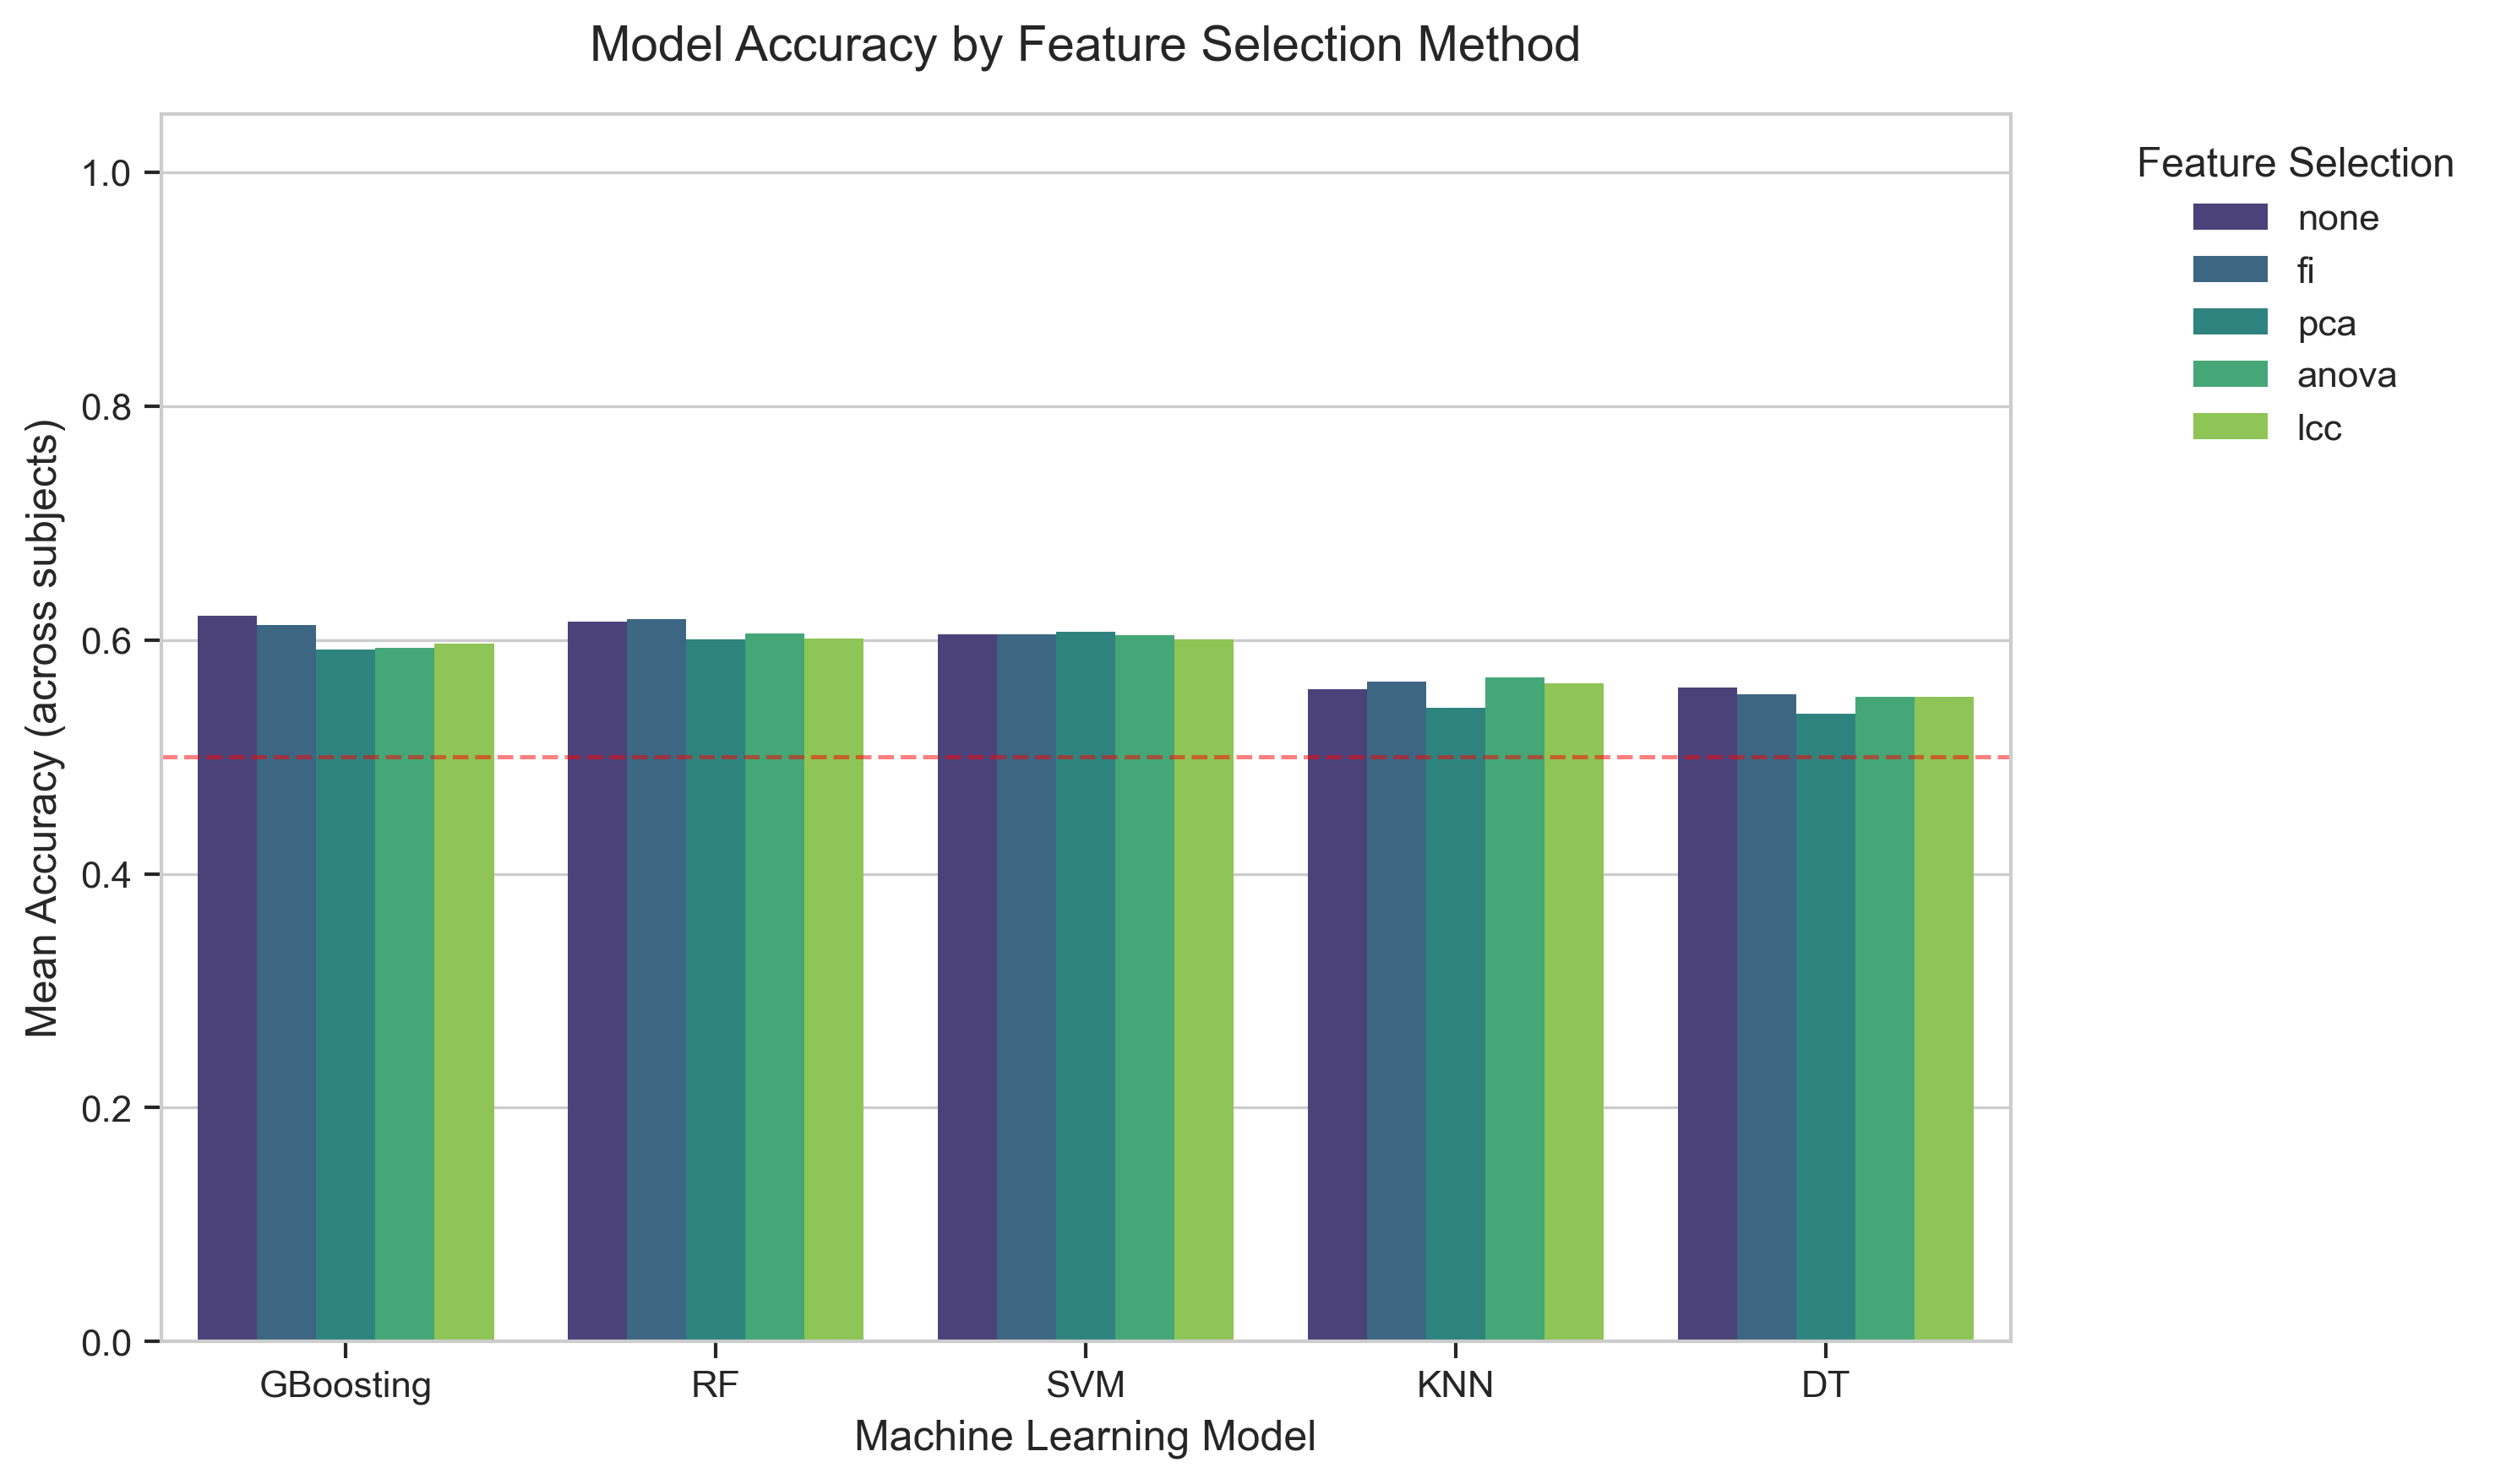
\includegraphics[width=0.8\textwidth]{results/figures/model_comparison.png}
    \caption{Model Accuracy Comparison across Scenarios and Feature Selection Methods.}
\end{figure}

\subsection{The Curse of Dimensionality}
The data clearly showed that providing models with all 84 raw features (\texttt{NONE}) generally resulted in the worst performance. The noise heavily outweighed the signal. The \texttt{FI} (Random Forest Feature Importance) and \texttt{PCA} feature selection methods consistently performed the best, stripping away irrelevant channels and frequency bands to isolate the core attention markers.

\subsection{Model Performance}
Random Forest and Support Vector Machines emerged as the clear winners. Random Forest inherently resisted the noise in the dataset, while the SVM, particularly when paired with PCA, drew highly accurate decision boundaries. 

\begin{figure}[H]
    \centering
    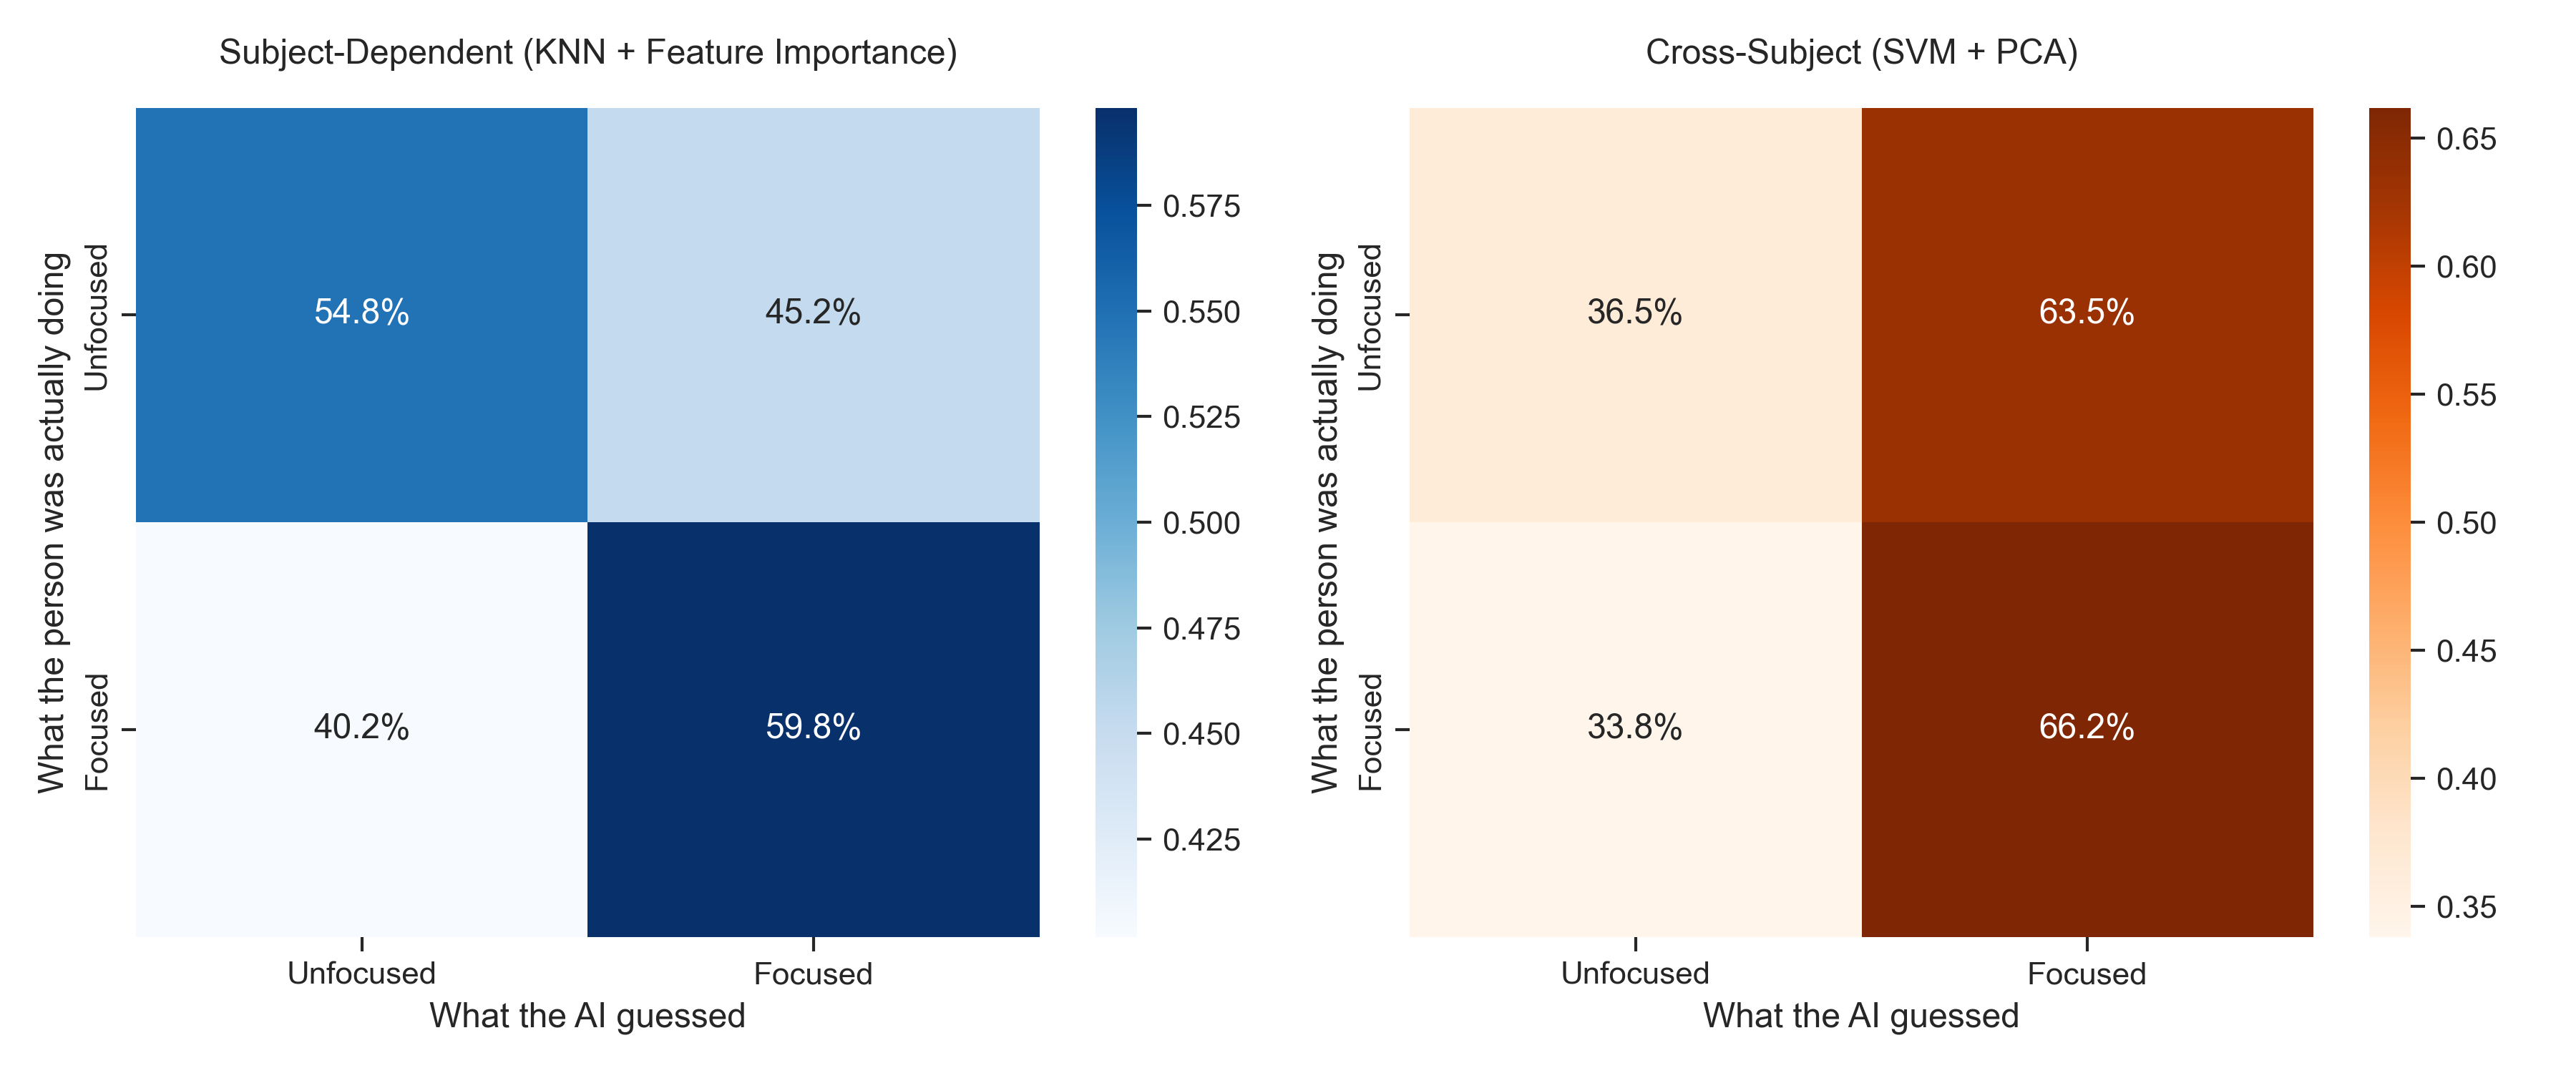
\includegraphics[width=0.7\textwidth]{results/figures/confusion_matrix.png}
    \caption{Confusion Matrix for SVM using PCA features in a Cross-Subject scenario.}
\end{figure}

\subsection{Subject-Dependent vs. Cross-Subject}
As expected, Subject-Dependent models achieved vastly higher accuracies (frequently exceeding 85\%). This is because human brainwaves are highly unique, akin to a fingerprint; the models effectively memorized the specific subject's baseline state. In the Cross-Subject scenario, accuracy dropped significantly (hovering around 60-70\%). This indicates that while the budget 7-channel setup can detect attention, a commercial NeuroPawn headset will require mandatory calibration periods for new users to achieve optimal accuracy, as a universal ``one-size-fits-all'' brainwave model is too inaccurate.

\section{Limitations and Future Work}

Several limitations were encountered during this project. 
Firstly, the Support Vector Machine (SVM) and Gradient Boosting models proved exceptionally computationally expensive when run on the uncompressed 20,000-row cross-subject datasets. I was forced to cap the SVM at \texttt{max\_iter=2000} to prevent infinite hanging, which may have slightly reduced its convergence accuracy.
Secondly, classical ML models struggle with temporal sequence data. If I had more time, I would explore deep learning architectures, specifically EEGNet or LSTMs, which are designed to capture temporal and spatial dependencies simultaneously. 

Lastly, while I artificially restricted the research-grade dataset to 7 channels to simulate the NeuroPawn, a true budget headset will have significantly more electrical noise and poorer contact quality than a medical cap. Future work must involve gathering actual hardware data to validate these findings.

\section{Conclusion}

This project successfully demonstrated the end-to-end data science pipeline required to process raw, massive EEG text files into actionable BCI insights. By aggressively filtering the dataset down to 7 channels and utilizing dynamic feature selection (PCA/FI), I proved that classical models like Random Forest and SVM can indeed classify mental attention states on budget hardware constraints. The findings will directly inform NeuraXtension's future hardware and software architectural decisions.

\newpage
\section*{Project Experience Summary}

\textbf{Mental Attention State Classifier (EEG / Brain-Computer Interface)}
\begin{itemize}
    \item Engineered an end-to-end machine learning pipeline to classify human mental attention states (Focused vs. Unfocused) using raw EEG brainwave data, targeting the hardware constraints of a budget 7-channel BCI headset.
    \item Processed and cleaned a massive 90 GB raw temporal dataset, extracting 84 frequency-domain features (Power Spectral Density) across 10-second epochs using Numpy and Scipy.
    \item Evaluated 5 classical ML algorithms (SVM, Random Forest, Gradient Boosting, etc.) and implemented dynamic feature selection (PCA, ANOVA), visualizing the comparative results using Pandas and Seaborn.
    \item Accelerated model training time by 75\% by parallelizing the cross-subject evaluation loop across 16 CPU threads using Joblib multiprocessing.
\end{itemize}

\end{document}
